\section{The Gibbs Sampler}

The Metropolis-Hastings Algorithm of the previous section can be difficult to apply when the dimension of the state space is high. 
The generation of the chain becomes too much of a multidimensional problem and becomes at least unwieldy, and possibly undoable.
Here Gibbs Sampler comes into play. The Gibbs Sampler is a spatial kind of Metropolis-Hastings Algorithm that very cleverly reduces the multidimensional problem into a sequence of \textit{one-dimensional} problem. 

Suppose a state $ \mathbf{x} $ in the state specs $ S $ is a vector in some $ m $-dimensional specs with $ \mathbf{x} = (x_1,x_2,x_3,\ldots,x_m) $. Suppose from current state $ \mathbf{x} $ we want to jump to a new state $ \mathbf{y}\in S $. According to Gibbs sampler we change coordinate one at a time,
such as $ (x_1,x_2,\ldots,x_m) \to (y_1,x_2,\ldots,x_m) \to (y_1,y_2,\ldots,x_m) \to \ldots \to (y_1,y_2,\ldots,y_m)  $, and each coordinate change is made by using the conditional distribution of that coordinate given the rest of the coordinates. 
For example, the transition $ (x_1,x_2,\ldots,x_m) \to (y_1,x_1,\ldots,x_m) $ is made by simulating from the distribution $ f(x_1|x_2,\ldots,x_m) $.
These conditional distribution of one coordinate gives all the rest are \textbf{full conditionals}. As, long as we can calculate and also simulate from all the full conditionals, a complicated multidimensional problem turns in to $ m $ one dimensional problems.

If current state $ \mathbf{x} = (x_1,x_2,x_3,\ldots,x_m)  $.Pick the coordinate to be changed at random from the $ m $ available coordinate. If the coordinate picked is $ i $, then the state $ \mathbf{y} = (x_1,x_2, \ldots , x_{j-1}, x , x_{j+1}, \ldots , x_m) $ work as a candidate state.
Then Gibbs sampler uses the Metropolis-Hastings algorithm with
\begin{align*}
    q(\mathbf{x},\mathbf{y}) &= \frac{1}{m} P( X_i = x | X_j = x_j, i\neq j )\\ 
                             &= \frac{f(\mathbf(y))}{mP(X_j = x_j, i \neq j)}
\end{align*}
Now the acceptance probability
\begin{align*}
    \alpha(\mathbf{x},\mathbf{y}) &= \min \left( \frac{f(\mathbf{y})q(\mathbf{y},\mathbf{x})}{f(\mathbf{x})q(\mathbf{x},\mathbf{y})} , 1 \right) \\ 
                                  &= \min \left(  \frac{ f(\mathbf{y})f(\mathbf{x}) }{  f(\mathbf{x})f(\mathbf{y})  } , 1  \right) \\ 
                                  &= 1
\end{align*}

Hence, Gibbs sampler is a special Metropolis-Hastings algorithm whose acceptance probability is always 1.

\subsection{Algorithm for Gibbs Sampler}
Suppose $ \mathbf{x}\in \mathds{R}^m $. Then algorithm of The Gibbs sampler can summarized as below:
\begin{enumerate}
    \item Set initial values $ \mathbf{x}^{(0)} = ( x_1^{(0)}, x_2^{(0)} , \ldots , x_m^{(0)}  ) $.
    \item Obtain a new value $ \mathbf{x}^{(j)} = ( x_1^{(j)}, x_2^{(j)}, \ldots , x_m^{(j)} )$ form $ x^{(j-1)} $ through \textit{full conditional distributions}
            \begin{align*}
                x_1^{(j)} &\sim f(x_1|x_2^{(j-1)}, \ldots, x_m^{(j-1)}  ),\\
                x_2^{(j)} &\sim f(x_2|x_1^{(j)}, x_3^{(j-1)}, \ldots, x_m^{(j-1)}), \\
                \vdots \\
                x_m^{(j)} &\sim f(x_m|x_1^{(j)}, \ldots , x_{m-1}^{(j)}  );
            \end{align*}
            \item Change counter $ j $ to $ j + 1 $ and return to step 2 until convergence is reached. 
\end{enumerate}

\subsection{Examples}
Now, we see some examples how to use Gibbs sampler.

\begin{example}[Generating standard bivariate normal distribution]

    In this example we try to generate standard bivariate normal distribution with correlation coefficient $ \rho $. Suppose,
    \[
        (X_1, X_2) \sim \text{N}\left(  
            \begin{bmatrix}
                0\\
                0
            \end{bmatrix},
            \begin{bmatrix}
                1 & \rho \\ 
                \rho & 1
            \end{bmatrix}
        \right)
    \]
    Where, $ \Sigma = \begin{bmatrix}
        1 & \rho \\ 
        \rho & 1
    \end{bmatrix} $ is known as \textbf{covariance matrix}.  Then, the probability density function of $ (X_1,X_2) $ would be,

    \[
        f(x_1,x_2) = \frac{1}{2 \pi \sqrt{1-\rho^2}} \exp \left( - \frac{1}{2(1-\rho^2)} (x^2 -2 \rho xy + y^2  ) \right)
    \]
    
    \begin{figure}[H]
        \centering
        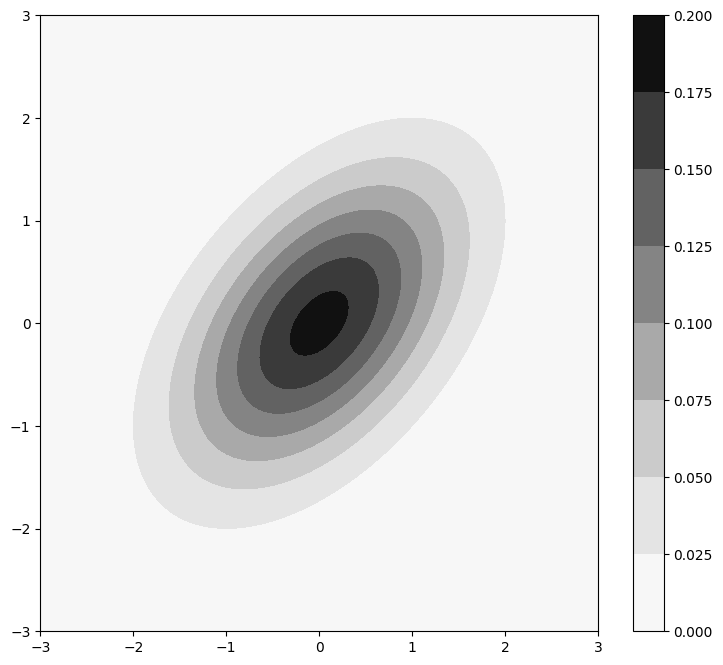
\includegraphics[width=0.6\textwidth]{images/gibbs/ex1-con-plot.png}
        \caption{Contour Plot of Bivariate Normal Distribution when $ \rho = 0.5 $}
    \end{figure}

    For using Gibbs Sampler we have to calculate $ f_{X_1|X_2}(x_1|x_2) $ and $ f_{X_2|X_1}(x_2|x_1) $.

    \begin{align*}
        f_{X_1|X_2}(x_1|x_2) &= \frac{f(x_1,x_2)}{f_{X_2}(X_2)} \\ 
                    &=C_1 f(x_1,x_2) \\
                    &=C_2 \exp \left( - \frac{1}{2 \sqrt{1-\rho^2}} (x_1^2 - 2 \rho x_1x_2) \right) \\
                    &= C_3 \exp \left(- \frac{1}{2 \sqrt{1-\rho^2}} (x_1 - \rho x_2)^2   \right)
    \end{align*}
     Recognizing this equation as a normal density, we can conclude that, 
     \[ X_1|X_2 \sim \text{N}(\rho x_2, (1-\rho^2)) \]

    Also, 
    \begin{align*}
        f_{X_2|X_1} (x_2|x_1) &= \frac{f(x_2,x_1)}{f_{X_1}(X_1)} \\ 
                    &=C_4 f(x_2,x_1) \\
                    &=C_5 \exp \left( - \frac{1}{2 \sqrt{1-\rho^2}} (x_2^2 - 2 \rho x_1x_2) \right) \\
                    &= C_6 \exp \left(- \frac{1}{2 \sqrt{1-\rho^2}} (x_2 - \rho x_1)^2   \right)
    \end{align*}
    Here also we can see that,
    \[
        X_2|X_1 \sim \text{N}\left(\rho x_1, (1-\rho^2)\right)
    \]

    So, the Gibbs sampler algorithm for this case would be,
    \begin{enumerate}
        \item Set an initial state $ \left(x_1^{(0)} , x_2^{(0)} \right) $
        \item We obtain the next state $ \left( x_1^{(t+1)} , x_2^{t+1} \right) $ through the full conditional distributions, 
            \begin{align*}
                x_1^{(t+1)} &\sim \text{N}\left(\rho x_2^{(t)}, (1-\rho^2) \right) \\
                x_2 ^{(t+1)} &\sim \text{N}\left(\rho x_1^{(t+1)}, (1-\rho^2) \right) 
            \end{align*}
    \end{enumerate}
    New we choosing different initial state we study the outputs.

    \textbf{Initial State 1:} Here we are taking initial state to be $(-1,-1)$. 
    \begin{figure}[H]
        \centering
        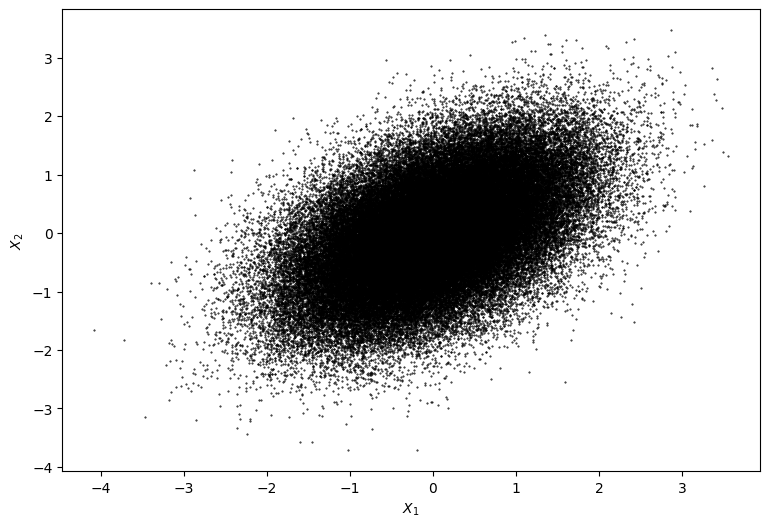
\includegraphics[width=0.5\textwidth]{images/gibbs/ex1-init1.png}
        \caption{Samples when initial state $(-1,-1)$}
    \end{figure}

    \textbf{Initial State 2:} Now we consider $(0,0)$ (middle of density) as a initial state. 

    \begin{figure}[H]
        \centering
        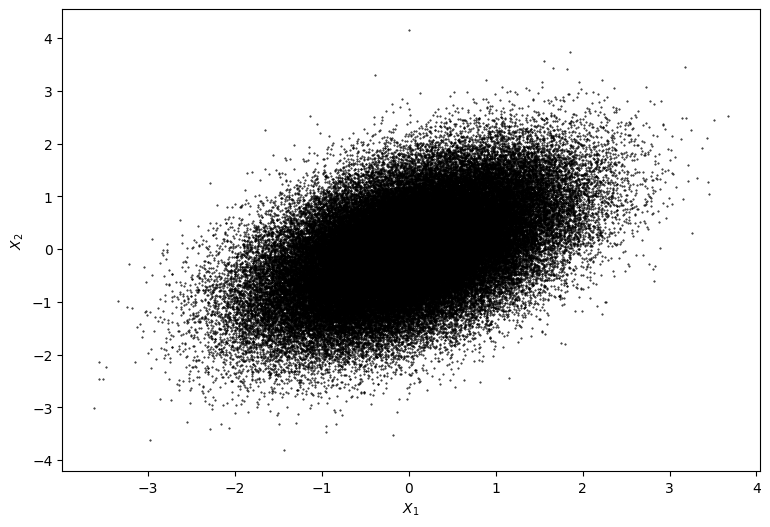
\includegraphics[width=0.5\textwidth]{images/gibbs/ex1-init2.png}
        \caption{Samples when initial state $(0,0)$}
    \end{figure}

    \textbf{Initial State 3:} Here we take initial state way out side form middle of distribution consider $ (-4,-4) $ as initial state. We can see from \Cref{fig:gb ex1 sample 3} although we are taking initial state way outside but the samples are come out to be same as above samples. 


    \begin{figure}[H]
        \centering
        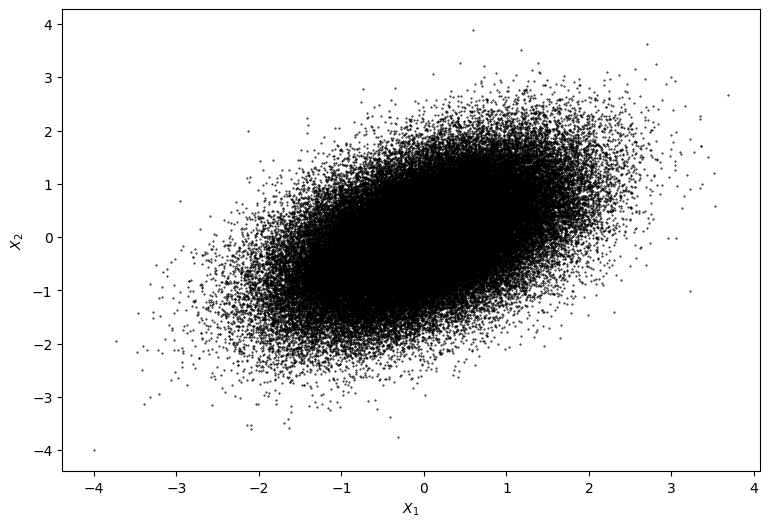
\includegraphics[width=0.5\textwidth]{images/gibbs/ex1-init3.png}
        \caption{Samples when initial state $(-4,-4)$}
        \label{fig:gb ex1 sample 3}
    \end{figure}

    \begin{figure}[H]
        \centering
        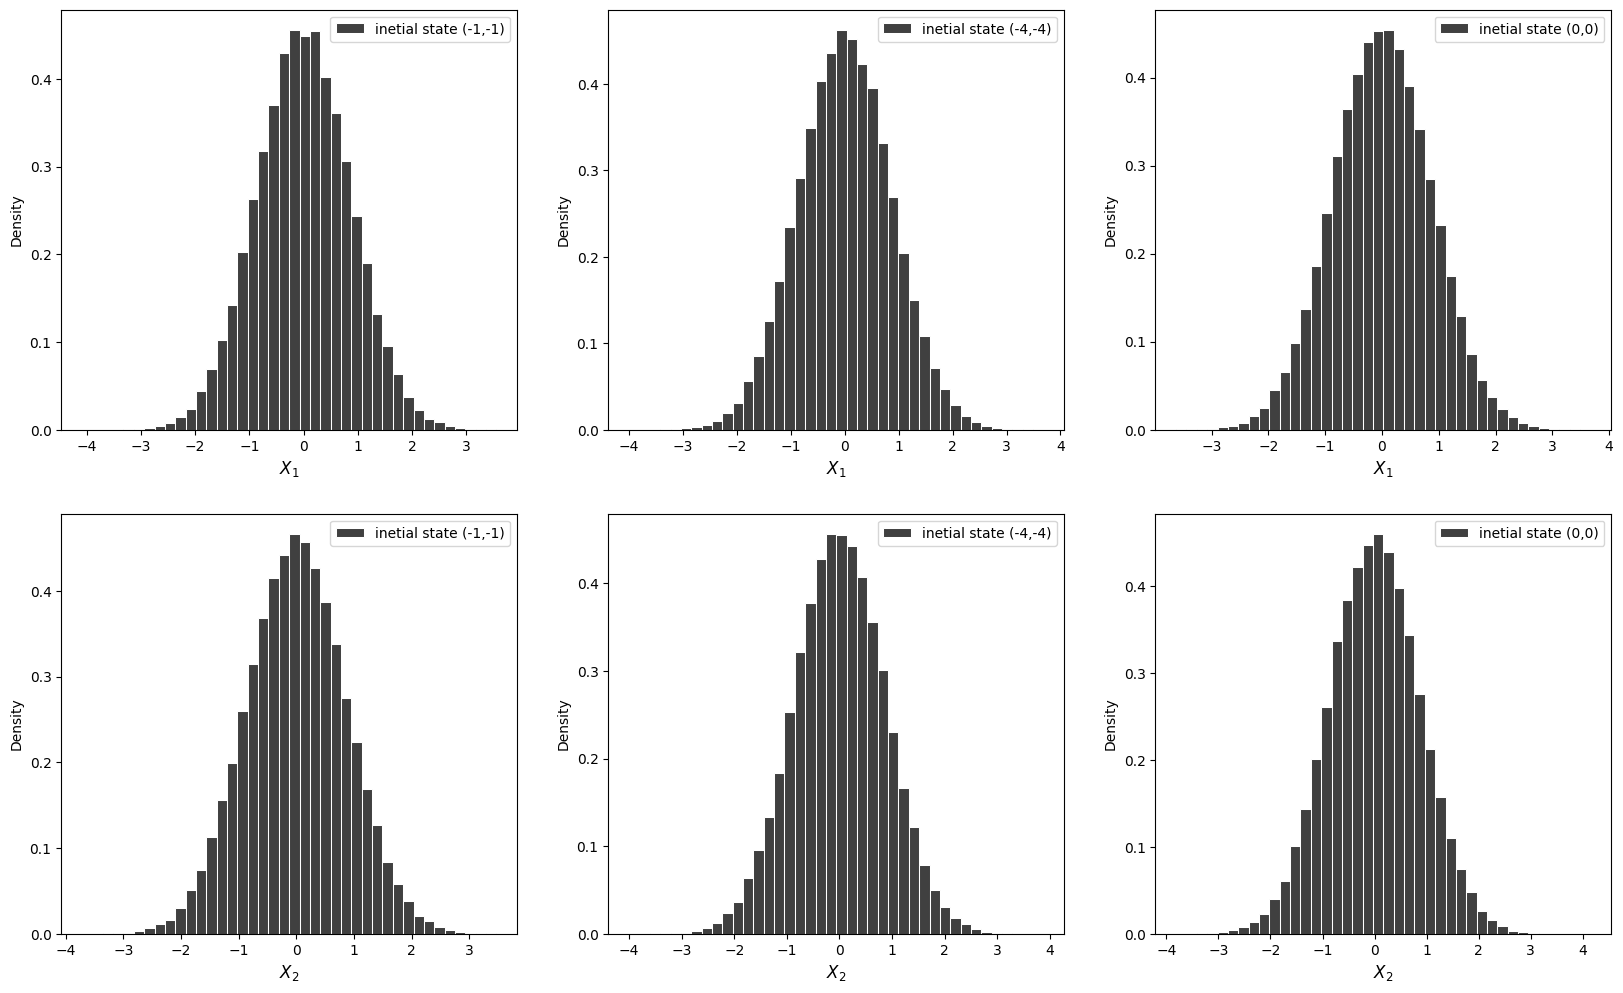
\includegraphics[width=1\textwidth]{images/gibbs/ex1-marginal-distributions.png}
        \caption{Marginal distribution for $ X_1 $ and $ X_2 $ for different initial states}
    \end{figure}

\end{example}

\begin{example}[Simulating Beta-Binomial Distribution]

    If $ X|p \sim \text{Bin}(n,p)$ for some fix $ n $, and $ p \sim \text{Beta}(\alpha,\beta) $, then the marginal distribution of $ X $ would be called a \textbf{Beta-Binomial distribution}.
    Its probability density function,
    \begin{align*}
        f_X(x) = \frac{\Gamma(\alpha+\beta)}{\Gamma(\alpha)\Gamma(\beta)} {n\choose x} \int_{0}^{1} p^{x + \alpha -1}(1-p)^{n - x + \beta -1}dp \ \ x = 0,1,2,\ldots,n  
    \end{align*}

    For simulating Beta-Binomial distribution using Gibbs sampler we have to simulate the pair $ (X,p) $ whose joint distribution is,
    \[
       f_{(X,p)}(x,p) = \frac{\Gamma(\alpha+\beta)}{\Gamma(\alpha)\Gamma(\beta)} {n\choose x} p^{x + \alpha -1}(1-p)^{n - x + \beta -1} , \, x = 0,1,2,\ldots,n, \, 0<p<1.  
    \]
    
    We know form definition of Beta-Binomial distribution,
    \[
        X|p \sim \text{Bin}(n,p)
    \]

    Now,
    \begin{align*}
        f_{p|X}(p|x) &= \frac{f(x,p)}{f(x)} \\ 
                &= \frac{ \frac{\Gamma(\alpha+\beta)}{\Gamma(\alpha)\Gamma(\beta)} {n\choose x} p^{x + \alpha -1}(1-p)^{n - x + \beta -1} }{ \frac{\Gamma(\alpha+\beta)}{\Gamma(\alpha)\Gamma(\beta)} {n\choose x} \int_{0}^{1} p^{x + \alpha -1}(1-p)^{n - x + \beta -1}dp } \\
                &= \frac{ p^{x + \alpha -1}(1-p)^{n - x + \beta -1} }{ \int_{0}^{1} p^{x + \alpha -1}(1-p)^{n - x + \beta -1}dp } \\
                &= \frac{ 1 }{ \text{Beta}(x+\alpha-1,n-x+\beta-1) } p^{x + \alpha -1}(1-p)^{n - x + \beta -1}
    \end{align*}
    Hence we have,
    \begin{equation}
        \label{eq:p|x}
        f_{p|X}(p|x) = \frac{\Gamma(\alpha+\beta+n)}{\Gamma(x+\alpha)\Gamma(n-x+\beta)} p^{x + \alpha -1}(1-p)^{n - x + \beta -1}
    \end{equation}

    Form \Cref{eq:p|x} we conclude that $ p|X\sim \text{Beta}(x+\alpha,n-x+\beta) $.

    So, the Gibbs sampler algorithm for this example,
    \begin{enumerate}
        \item Choose an initial state $ p^{(0)} \sim \text{Beta}(\alpha,\beta)  $.
        \item Obtain the next state $ \left(x^{(t+1)}, p^{(t+1)}\right) $ through the full conditional distributions,
            \begin{align*}
                x^{(t+1)} &\sim \text{Bin}\left( n,p^{(t)} \right),\\
                p^{(t+1)} &\sim \text{Beta}\left(x^{(t+1)}+\alpha, n-x^{(t+1)}+\beta \right) 
            \end{align*}
        \item Replete step 2.  
    \end{enumerate}

    Now, taking $ n=10,\,\alpha=7,\,\beta=2 $ we simulate beta-binomial distribution and we get empirical mean 7.7797, variance 3.2788 which are close to theoretical mean($ \mu $) and variance($ \sigma^2 $).
    \begin{align*}
        \mu &= \frac{n \alpha}{\alpha+\beta} = \frac{10 \times 7 }{ 7 + 2} = 7.7777 \\
        \sigma^2 &= \frac{n \alpha \beta(\alpha+\beta+n)}{(\alpha+\beta)^2(\alpha+\beta+1)} = 3.2840
    \end{align*}
    
    \begin{figure}[H]
        \centering
        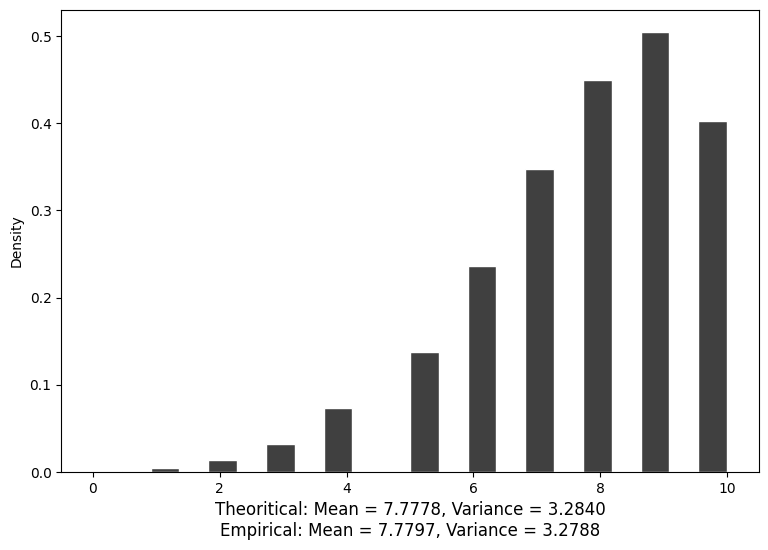
\includegraphics[width=0.6\textwidth]{images/gibbs/ex2-beta-binomial.png}
        \caption{Simulation of Beta-Binomial(10,7,2)}
        \label{fig:beta-binomial simulation}
    \end{figure}

\end{example}



